\chapter{Results}
\label{ch:results}

This chapter presents the experimental results of the Seriguela pipeline, following the phased design of Section~\ref{sec:design}. We first summarize the preliminary experiments and the methodological lessons that shaped the final protocol (Section~\ref{sec:prephase}). We then report the zero-shot model selection (Section~\ref{sec:phase1_results}), the stability findings from the pilot study (Section~\ref{sec:stability_findings}), and the controlled five-arm comparison with its statistical analysis (Section~\ref{sec:phase2_results}). Finally, the champion configuration faces the 122-problem SRBench challenge (Section~\ref{sec:phase4_results}). Unless stated otherwise, every number in this chapter comes from the versioned per-seed result files in the project repository.

\section{Preliminary Experiments and Methodological Lessons}
\label{sec:prephase}

Two rounds of preliminary experimentation preceded the final protocol, and both left marks on its design.

The first round was a set of 36 exploratory RL runs (4 algorithms $\times$ 3 problems $\times$ 3 seeds) on the Base Infix model. Its headline observation --- that every algorithm solves Nguyen-1 with $R^2 \geq 0.99$, making the problem useless for discrimination --- led to Nguyen-1's exclusion from the main comparison. The same data, however, contained a subtle flaw: the BoN arms had been launched with the SR-IC reward while the pure arms used clipped $R^2$. Any BoN-versus-pure comparison on these runs would confound the buffer with the reward. The final protocol's insistence on a \emph{uniform} reward across arms descends directly from this experience.

\label{sec:phase_a_lessons}
The second round was far larger --- a factorial sweep of roughly 9{,}700 runs over models, problems, algorithms, rewards, penalties, temperatures, prompts, and noise levels --- and it failed. A post-hoc audit found four disqualifying defects: (i) the Best-of-N baseline had crashed silently in \emph{every} run due to a type-mismatch bug, reporting $R^2 = 0$ and invalidating all comparative claims; (ii) 89\% of the configurations had been run with a single seed, making it impossible to distinguish robust configurations from lucky ones; (iii) the factorial grid was fragmented, with 280 combinations missing entirely, so marginal means were biased toward whichever configurations happened to complete; and (iv) the reward and penalty settings of thousands of runs were not correctly logged. The dataset was discarded.

Three design rules were extracted from this failure and applied to everything that follows: \textbf{replication before breadth} (five seeds per cell, even if it means fixing auxiliary factors); \textbf{baselines must demonstrably run} (the Best-of-N arm was re-implemented and its output verified end to end); and \textbf{process metrics are recorded at every step} (validity rate, KL divergence, memory footprint), because final scores alone cannot reveal a silently broken experiment. The pilot findings of Section~\ref{sec:stability_findings} vindicate the third rule directly.

\section{Phase 1 --- Zero-Shot Model Selection}
\label{sec:phase1_results}

Phase 1 asks which fine-tuned model should carry the expensive RL phases. Both Infix candidates --- Base (124M) and Large (774M) --- attempted all 122 benchmark problems by pure sampling (Best-of-N, $N=512$, 10 seeds per problem).

\begin{figure}[htbp]
    \centering
    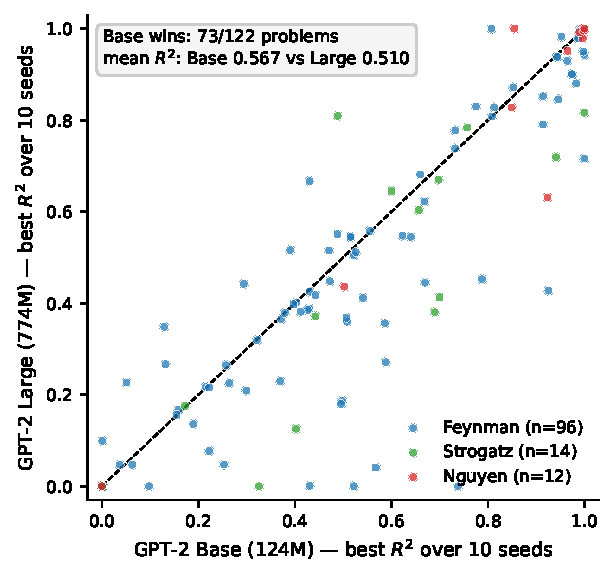
\includegraphics[width=0.72\linewidth]{figures/fig_zero_shot_selection.pdf}
    \caption[Zero-shot model selection: Base vs.\ Large]{Zero-shot comparison on the 122 benchmark problems (best $R^2$ over 10 seeds of Best-of-N sampling, $N=512$). Each point is one problem; points below the diagonal favor the smaller model. Base wins on 73 of 122 problems and on the mean.}
    \label{fig:zero_shot}
\end{figure}

Figure~\ref{fig:zero_shot} summarizes the outcome. Against the intuition that larger is better, the Base model \emph{wins}: its mean best $R^2$ across problems is 0.567 versus 0.510 for Large (medians 0.534 versus 0.450), and it is the better model on 73 of the 122 problems. The Large model shows a slightly higher raw validity rate (94.2\% versus 92.1\% of sampled expressions parse and evaluate), but this small syntactic advantage does not translate into better discoveries. A plausible reading is that at this scale and with this amount of fine-tuning data, the extra capacity of GPT-2 Large mostly sharpens the SFT prior rather than broadening it --- and a sharper prior samples a narrower slice of expression space.

The decision followed the pre-registered criterion: \textbf{Base Infix} (124M) carries all subsequent phases, at roughly 40\% of the compute cost of the alternative. The Infix notation was fixed for the RL phases --- all preliminary RL evidence had been collected in this notation --- and the Prefix models are released as public artifacts for future work.

\section{Pilot Findings: Three Silent Failure Modes}
\label{sec:stability_findings}

Before committing the compute budget of the main experiment, short pilot runs ($\sim$US\$2 of GPU time in total) probed the protocol end to end. They surfaced three failure modes, each invisible to final-score metrics, each capable of silently invalidating the entire experiment.

\subsection{The Reward Dead Zone}
\label{sec:deadzone}

The original protocol called for the SR-IC reward (Table~\ref{tab:reward_functions}) as the uniform training signal. The pilot revealed that, under the $C=1$ protocol, SR-IC has a \emph{dead zone}: its clipped normalization zeroes the reward of essentially every expression the model can reach --- any candidate whose complexity penalty exceeds its fit term scores exactly zero. Figure~\ref{fig:deadzone} shows the consequence. A 500-step Pure-PPO run under SR-IC ($\approx$512K sampled expressions) received a strictly non-positive mean reward at every single step (panel a): the gradient signal never distinguished a promising expression from a useless one. Its best-$R^2$ curve (panel b) is correspondingly flat --- the early rise is pure sampling luck, after which 470 steps of ``training'' produce nothing. Under clipped $R^2$, the same algorithm on the same problem receives a dense, informative signal and climbs to an exact solution.

\begin{figure}[htbp]
    \centering
    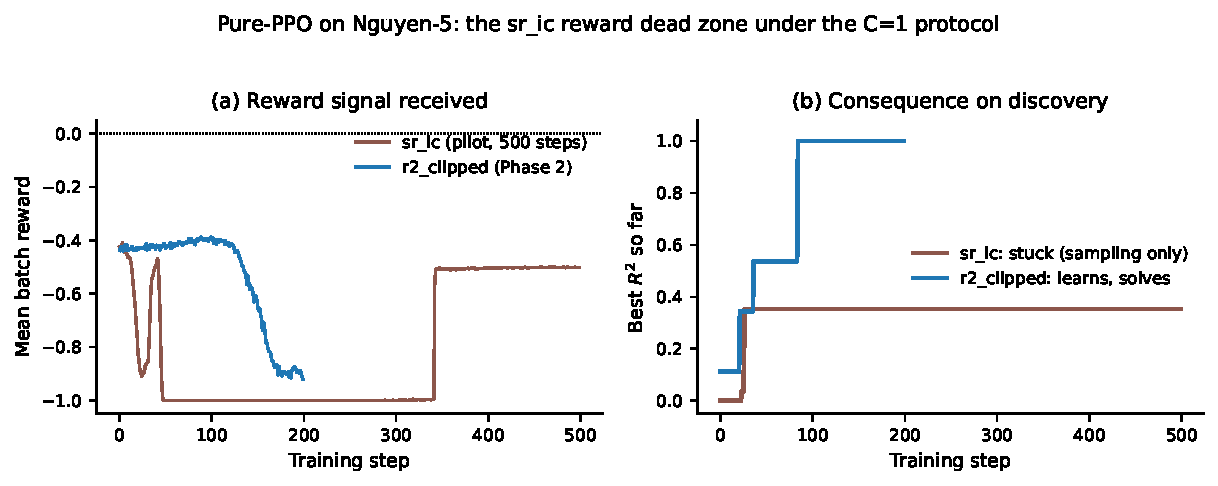
\includegraphics[width=0.95\linewidth]{figures/fig_sric_deadzone.pdf}
    \caption[The SR-IC reward dead zone]{The SR-IC reward dead zone (Pure-PPO on Nguyen-5). (a) Mean batch reward per step: under SR-IC the model never receives a positive signal; under clipped $R^2$ the signal is dense. (b) Best $R^2$ found so far: SR-IC stalls at its sampling luck; clipped $R^2$ learns and solves the problem.}
    \label{fig:deadzone}
\end{figure}

Beyond forcing the switch to clipped $R^2$ as the uniform reward, the dead zone reinterprets the preliminary data of Section~\ref{sec:prephase}: the BoN arms of that round, which ran under SR-IC, were effectively performing Best-of-N sampling with an elite buffer --- their policy-gradient component was receiving no usable signal. It also carries a general lesson for reward design in symbolic regression: a reward that is theoretically well-motivated (information criteria have impeccable pedigree) can still be \emph{operationally} dead in the region of expression space the policy actually visits.

\subsection{PPO Policy Collapse at Shared Defaults}
\label{sec:ppo_collapse}

With the reward fixed, a second pilot probed update stability. At the framework defaults --- learning rate $1\times10^{-5}$, 4 PPO epochs per batch, max KL 0.1 --- the PPO update destroyed its own policy within ten steps: expression validity fell from the SFT prior's 59\% to 0\% and never recovered, with the per-epoch KL divergence reaching 0.22 in a single epoch. The mechanism is autocatalytic: an aggressive update damages the delicate token distributions that produce valid syntax; invalid expressions then earn uniform penalties, whose gradients further scramble the policy. The elite buffer cannot prevent this --- the defect is in the update, not the data mix --- so both PPO arms (pure and BoN) collapsed identically.

A conservative recipe --- learning rate $1\times10^{-6}$, 2 epochs, max KL 0.02 --- restored stable training; under it, Pure-PPO solved Nguyen-5 exactly ($R^2 = 1.0$ at step 57 of a pilot run) where Best-of-N plateaus at $\approx$0.39. GRPO, in contrast, ran stably at the shared defaults --- its rank-based group advantages are inherently robust to reward scale, and validity recovered above 90\% without intervention. The main experiment therefore uses tuned updates for the PPO arms and defaults for GRPO, an asymmetry reported as a finding: \textbf{in this regime, PPO requires careful update tuning to function at all, while GRPO does not}. Since GRPO received no problem-specific tuning, it enjoys the conservative side of the comparison.

\subsection{Evaluator Memory Blow-Up}

The third failure mode was infrastructural. SymPy's internal caches grow monotonically as millions of distinct expressions are parsed and simplified; over a long run, the process footprint grew to $\approx$38~GB and the container was killed. Periodic cache flushes resolved the leak for most arms, but the BoN-GRPO arm --- whose buffer keeps re-injecting long expressions that GRPO's updates tend to elongate further --- additionally required the complexity cap and the anti-hang watchdog described in Section~\ref{sec:guards} to become executable on the polynomial problems. With the guards in place, all twenty cells of the design completed.

The three findings share a moral: none of them is visible in a leaderboard of final $R^2$ scores. A run with a dead reward, a collapsed policy, or a crashed evaluator still \emph{terminates} and still \emph{reports a number}. Only step-level process metrics --- mean reward, validity rate, KL divergence, memory --- distinguish a healthy experiment from a hollow one. We consider this instrumentation requirement a first-class methodological contribution of the thesis.

\section{Phase 2 --- Controlled Comparison of the Five Arms}
\label{sec:phase2_results}

The main experiment ran the five arms of Table~\ref{tab:rl_algorithms} on Nguyen-3, 5, 7, and 9, with five seeds per cell --- 100 seed-runs, all completed, every arm consuming the same budget of $\approx$205K sampled expressions per seed. Table~\ref{tab:phase2_master} reports the full results; Figure~\ref{fig:phase2_box} shows the per-seed distributions.

\begin{table}[htbp]
    \centering
    \caption[Phase 2 master results]{Phase 2 results: best $R^2$ over 5 seeds (mean $\pm$ SD and median), exact discoveries (seeds reaching the SRBench criterion $R^2 > 0.999$), and complexity of the best expression (tokens). All arms share reward, budget, and seeds.}
    \label{tab:phase2_master}
    \small
    \begin{tabular}{llcccc}
    \toprule
    \textbf{Problem} & \textbf{Arm} & \textbf{Best $R^2$ (mean$\pm$SD)} & \textbf{Median} & \textbf{Exact} & \textbf{Compl.} \\
    \midrule
    Nguyen-3 & Best-of-N & $0.998 \pm 0.001$ & 0.998 & 0/5 & 12 \\
             & Pure-PPO  & $0.992 \pm 0.007$ & 0.995 & 0/5 & 16 \\
             & Pure-GRPO & $0.985 \pm 0.007$ & 0.985 & 0/5 & 18 \\
             & BoN-PPO   & $0.996 \pm 0.005$ & 0.998 & 1/5 & 15 \\
             & BoN-GRPO  & $0.997 \pm 0.002$ & 0.998 & 0/5 & 20 \\
    \midrule
    Nguyen-5 & Best-of-N & $0.626 \pm 0.020$ & 0.629 & 0/5 & 13 \\
             & Pure-PPO  & $0.755 \pm 0.249$ & 0.845 & 2/5 & 16 \\
             & Pure-GRPO & $0.268 \pm 0.236$ & 0.113 & 0/5 & 17 \\
             & BoN-PPO   & $\mathbf{0.857 \pm 0.286}$ & \textbf{1.000} & \textbf{4/5} & 14 \\
             & BoN-GRPO  & $0.278 \pm 0.212$ & 0.223 & 0/5 & 18 \\
    \midrule
    Nguyen-7 & Best-of-N & $0.999 \pm 0.000$ & 0.999 & 1/5 & 12 \\
             & Pure-PPO  & $0.998 \pm 0.000$ & 0.999 & 0/5 & 12 \\
             & Pure-GRPO & $0.999 \pm 0.000$ & 0.999 & 0/5 & 11 \\
             & BoN-PPO   & $0.999 \pm 0.000$ & 0.999 & 1/5 & 14 \\
             & BoN-GRPO  & $0.999 \pm 0.000$ & 0.999 & 4/5 & 19 \\
    \midrule
    Nguyen-9 & Best-of-N & $0.790 \pm 0.018$ & 0.788 & 0/5 & 11 \\
             & Pure-PPO  & $0.737 \pm 0.247$ & 0.788 & 2/5 & 13 \\
             & Pure-GRPO & $0.666 \pm 0.187$ & 0.546 & 0/5 & 15 \\
             & BoN-PPO   & $\mathbf{0.825 \pm 0.088}$ & 0.788 & 1/5 & 14 \\
             & BoN-GRPO  & $0.701 \pm 0.125$ & 0.794 & 0/5 & 15 \\
    \bottomrule
    \end{tabular}
\end{table}

\begin{figure}[htbp]
    \centering
    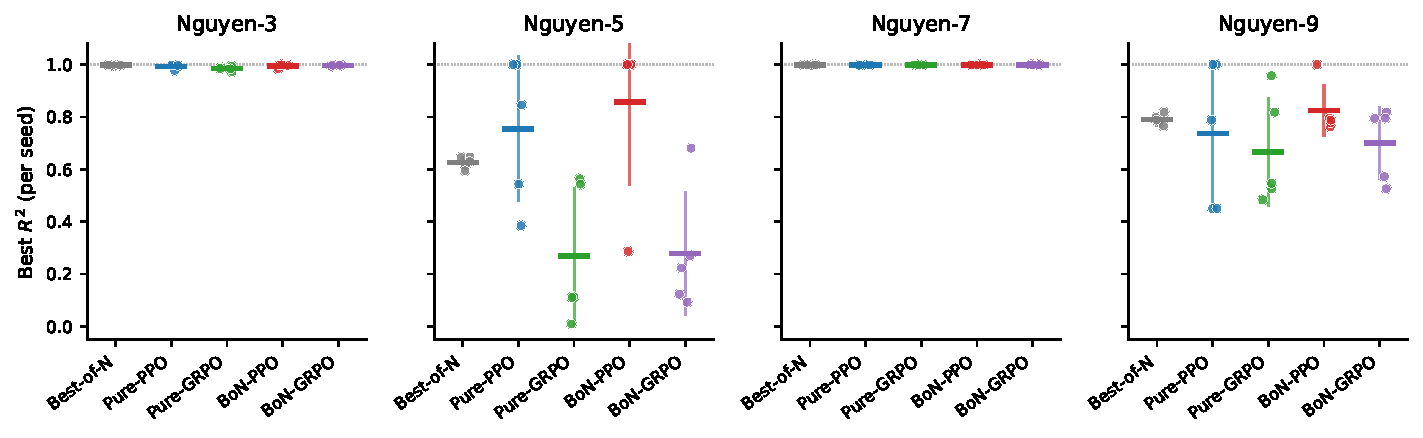
\includegraphics[width=0.99\linewidth]{figures/fig_phase2_box.pdf}
    \caption[Phase 2 per-seed distributions]{Per-seed best $R^2$ by arm and problem (points: seeds; bar: mean; whisker: $\pm$1 SD). Nguyen-3 and Nguyen-7 are saturated --- every arm reaches $R^2 \approx 0.99$ --- and act as sanity checks. The separation appears on Nguyen-5, the needle-in-a-haystack problem, and more mildly on the two-variable Nguyen-9.}
    \label{fig:phase2_box}
\end{figure}

\subsection{Overall Picture}

Two of the four problems (Nguyen-3 and Nguyen-7) turn out to be \emph{saturated}: every arm, including the no-learning baseline, reaches $R^2 \approx 0.99$, so they carry no discriminative signal about mean performance --- their role reduces to confirming that no arm is broken. (They do retain signal about \emph{exact} discovery: on Nguyen-7, notably, BoN-GRPO converts near-perfect fits into the exact expression in 4/5 seeds, more than any other arm.)

The informative problem is \textbf{Nguyen-5} ($\sin(x^2)\cos(x) - 1$), a target whose structure is rare under the SFT prior --- a needle in a haystack. Here the arms separate widely: BoN-PPO finds the \emph{exact} symbolic solution in 4 of 5 seeds (mean $0.857$, median $1.0$); Pure-PPO finds it in 2 of 5 ($0.755$); the baseline plateaus at $0.626$ and never finds it; and both GRPO arms collapse to local optima around $0.27$. On Nguyen-9 (two variables), the ordering repeats more mildly, with BoN-PPO again on top ($0.825 \pm 0.088$) and, notably, the smallest variance of any RL arm.

The Best-of-N baseline --- given the identical sampling budget --- bounds the contribution of learning itself: on Nguyen-5, the policy gradient plus buffer adds $+0.23$ of mean best $R^2$ and $+80$ percentage points of exact-discovery rate over pure sampling. This answers \textbf{RQ1} affirmatively, with a caveat the saturated problems make explicit: RL earns its cost only where the prior does not already solve the problem.

\subsection{Convergence and the Validity Valley}

\begin{figure}[htbp]
    \centering
    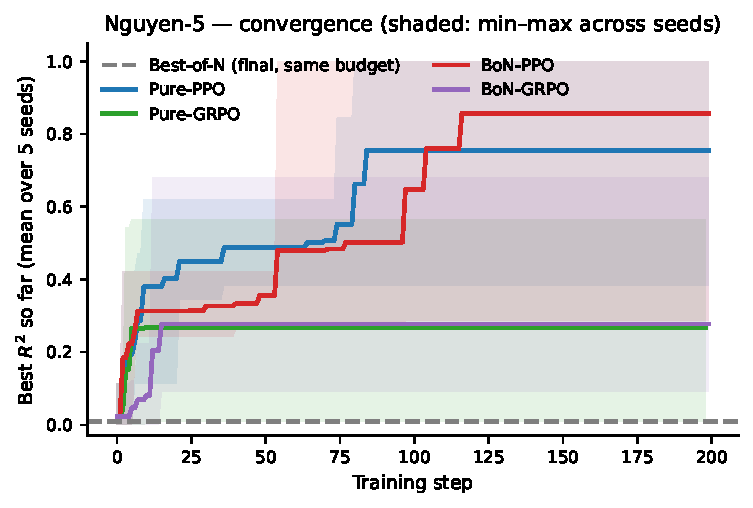
\includegraphics[width=0.78\linewidth]{figures/fig_phase2_convergence.pdf}
    \caption[Convergence on Nguyen-5]{Convergence on Nguyen-5: best $R^2$ found so far, averaged over 5 seeds (bands: min--max). The GRPO arms freeze within $\approx$15 steps; the PPO arms keep discovering throughout the run. The dashed line is the Best-of-N baseline at the same total budget.}
    \label{fig:phase2_convergence}
\end{figure}

Figure~\ref{fig:phase2_convergence} shows \emph{when} discoveries happen. The GRPO arms converge almost immediately --- their best expression is typically found before step 15 and never improves again. The PPO arms behave differently: discoveries continue throughout the 200 steps, with the BoN-PPO mean climbing in visible jumps as individual seeds hit the exact solution (steps $\approx$55, 100, 116). The step of best discovery, recorded per seed, confirms the pattern across all problems (Table~\ref{tab:phase2_master} reports it implicitly through the exact counts): GRPO's median best-step is in the single digits; PPO's ranges from 44 to 198.

\begin{figure}[htbp]
    \centering
    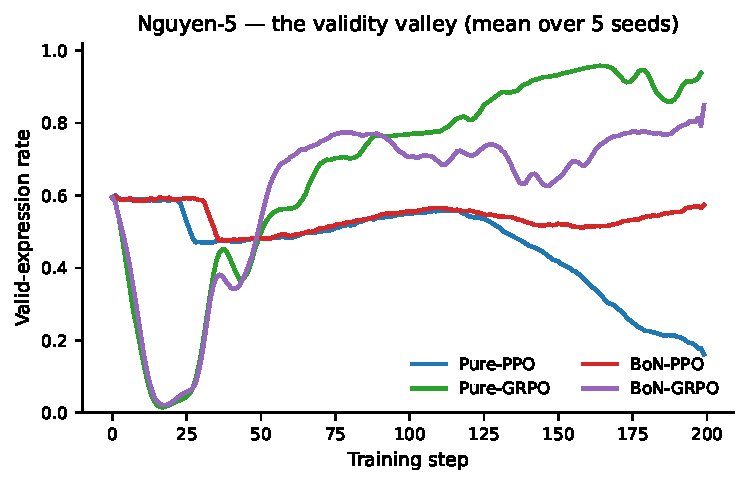
\includegraphics[width=0.78\linewidth]{figures/fig_phase2_validity.pdf}
    \caption[The validity valley on Nguyen-5]{The validity valley (Nguyen-5, mean over 5 seeds). Every RL arm initially ``forgets'' how to write valid expressions as the first updates perturb the SFT prior ($\approx$59\% validity), bottoming out near zero around steps 10--30. GRPO recovers to $>$90\%; BoN-PPO stabilizes near 55\%; Pure-PPO drifts down to $\approx$20\% by the end of the run.}
    \label{fig:phase2_validity}
\end{figure}

The validity dynamics (Figure~\ref{fig:phase2_validity}) explain the difference. Every RL arm dives into a \emph{validity valley} at the start of training --- the first policy updates perturb the fragile token distributions responsible for syntax, and the fraction of parseable expressions collapses from the prior's 59\% to nearly zero before recovering. What distinguishes the arms is where they \emph{stabilize}. GRPO climbs back above 90\%: its updates are gentle, and the policy settles into the high-probability modes of the prior --- syntactically pristine, structurally conservative. The PPO arms never fully recover, hovering between 20\% and 60\% validity for the entire run. Crucially, this is not a defect to be tuned away: operating near the edge of syntactic instability is functionally a regime of broad stochastic search, and it is exactly the PPO arms that keep discovering new expressions late into training. The depth-of-valley/breadth-of-search connection is quantified next.

\subsection{The Mechanism: Exploration $\times$ Retention}
\label{sec:mechanism}

\begin{figure}[htbp]
    \centering
    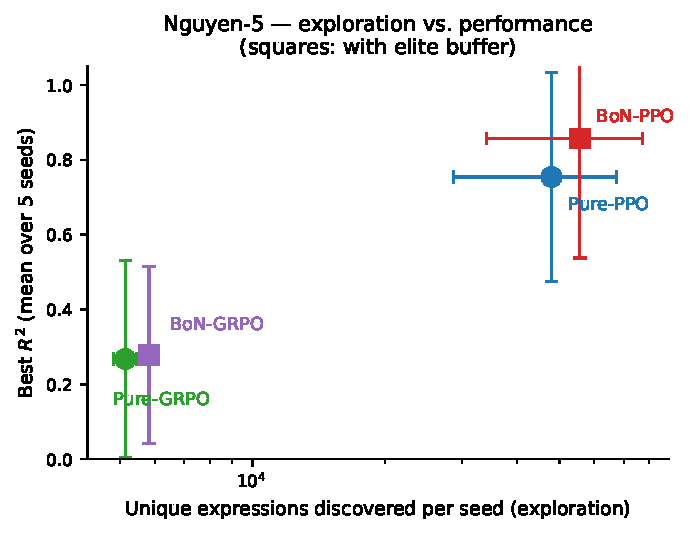
\includegraphics[width=0.7\linewidth]{figures/fig_phase2_exploration.pdf}
    \caption[Exploration vs.\ performance on Nguyen-5]{Exploration versus performance on Nguyen-5. Exploration is measured as unique expressions discovered per seed (log scale); squares mark the arms with an elite buffer. The PPO arms explore an order of magnitude more widely than the GRPO arms; the buffer converts Pure-PPO's discoveries into retained performance (BoN-PPO), but has nothing to retain in the GRPO regime (BoN-GRPO $\approx$ Pure-GRPO).}
    \label{fig:phase2_exploration}
\end{figure}

Why does BoN-PPO win, and why does the same buffer do nothing for GRPO? The process metrics decompose the answer into two orthogonal factors.

\textbf{Exploration} --- how much of expression space a run visits --- is a property of the update algorithm. Counting unique expressions discovered per seed, the PPO arms explore roughly \textbf{an order of magnitude more} than the GRPO arms ($\approx$35--56K versus $\approx$4--7K unique expressions on Nguyen-5). The mechanism traces back to the advantage computation: GRPO normalizes advantages by rank within each group, and when most of a group earns similar (often zero) reward, the selective pressure shrinks --- the policy settles early into the prior's high-probability modes and stops searching. PPO's tuned-but-aggressive updates keep the policy near the edge of instability, in the meta-stable low-validity regime seen above, which functions as a wide stochastic search.

\textbf{Retention} --- whether a rare, high-quality discovery survives --- is what the elite buffer provides. Pure-PPO demonstrates the failure mode it fixes: the arm \emph{found} the exact solution in more seeds than it ultimately \emph{kept} progressing from, because a discovery that appears once in a batch is diluted by the next update. The buffer re-injects elites as a persistent gradient anchor (in the spirit of DSR's Priority Queue Training \cite{petersen2020deep}), converting transient luck into stable convergence: 4/5 exact solutions for BoN-PPO versus 2/5 for Pure-PPO.

The decomposition makes a falsifiable prediction: \emph{the buffer should help only the arm that already explores}. In the GRPO regime, there are almost no rare high-$R^2$ discoveries to retain, so adding the buffer should change nothing --- and indeed BoN-GRPO $\approx$ Pure-GRPO on every problem (Table~\ref{tab:phase2_master}; Figure~\ref{fig:phase2_exploration}). Each of the five arms lands where the two-factor account predicts: the baseline has neither factor (sampling ceiling); Pure-PPO explores but forgets (bimodal outcomes); Pure-GRPO neither explores nor needs retention (early freeze); BoN-GRPO retains an empty treasury; BoN-PPO --- the only arm with both factors --- is the only arm that solves the needle problem reliably. This mechanism is the thesis's answer to \textbf{RQ2} and \textbf{RQ3}: the elite buffer helps \emph{conditionally on exploration}, and PPO versus GRPO differ not primarily in final $R^2$ but in the exploration regime their updates induce.

\subsection{Formal Statistics}
\label{sec:phase2_stats}

Table~\ref{tab:anova} reports the per-problem one-way ANOVA over best $R^2$ (5 seeds per arm) with Tukey HSD post-hoc contrasts and Cohen's $d$ for the significant pairs.

\begin{table}[htbp]
    \centering
    \caption[ANOVA and post-hoc tests for Phase 2]{Per-problem ANOVA over best $R^2$ and significant Tukey HSD contrasts (adjusted $p < 0.05$) with Cohen's $d$.}
    \label{tab:anova}
    \small
    \begin{tabular}{llll}
    \toprule
    \textbf{Problem} & \textbf{ANOVA} & \textbf{Significant contrasts (Tukey HSD)} & \textbf{Cohen's $d$} \\
    \midrule
    Nguyen-3 & $F=3.68$, $p=0.021$ & Best-of-N $\times$ Pure-GRPO & $+2.4$ \\
             &                     & Pure-GRPO $\times$ BoN-GRPO   & $-2.2$ \\
    \midrule
    Nguyen-5 & $F=6.05$, $p=0.002$ & Pure-PPO $\times$ Pure-GRPO   & $+2.0$ \\
             &                     & Pure-PPO $\times$ BoN-GRPO    & $+2.1$ \\
             &                     & Pure-GRPO $\times$ BoN-PPO    & $-2.2$ \\
             &                     & BoN-PPO $\times$ BoN-GRPO     & $+2.3$ \\
    \midrule
    Nguyen-7 & $F=3.37$, $p=0.029$ & Pure-PPO $\times$ BoN-GRPO    & $-2.3$ \\
    \midrule
    Nguyen-9 & $F=0.69$, $p=0.61$  & none & --- \\
    \bottomrule
    \end{tabular}
\end{table}

On the discriminative problem (Nguyen-5), the omnibus test is strongly significant ($p=0.002$) and all four significant pairwise contrasts point the same way: the PPO arms dominate the GRPO arms with very large effects ($|d| \geq 2.0$). On the saturated problems the significant contrasts involve differences of a few thousandths of $R^2$ --- statistically detectable because the within-arm variance is tiny, but practically irrelevant. Nguyen-9 shows no significant separation, consistent with its overlapping distributions.

Two caveats temper the parametric analysis. With $n=5$ per cell, power reaches 80\% only for effects of $d \gtrsim 1.5$ --- adequate here, since the effects of interest are of exactly that magnitude, but small and moderate differences remain undetectable. And the outcome distributions of the PPO arms are bimodal (a seed either finds the exact solution or stalls at a local optimum), violating ANOVA's normality assumption; for this reason we lean on the \emph{exact-discovery rate} (4/5 vs.\ 0/5 with a Wilson binomial interval) as the primary evidence on Nguyen-5, with the ANOVA in a supporting role, and non-parametric checks (Kruskal--Wallis) agree with the reported conclusions.

\subsection{What the Model Actually Found}

Beyond the numbers, the discovered expressions themselves carry evidence. The exact solutions to Nguyen-5 ($\sin(x^2)\cos(x)-1$) arrived in several algebraically equivalent but syntactically distinct forms:

\begin{itemize}
    \item Pure-PPO: \ \texttt{sin(x\_1*x\_1)*cos(x\_1) - C} \quad and \quad \texttt{sin(x\_1**C)*cos(x\_1) - C}
    \item BoN-PPO: \ \texttt{cos(x\_1)*sin(x\_1*x\_1) - C}, \quad \texttt{sin(x\_1/C*x\_1)*cos(x\_1) - C}, \\ \hspace*{1.55cm}\texttt{sin(x\_1*x\_1)*cos(x\_1) - C}
\end{itemize}

With $C=1$, all five reduce to the target. The variety matters: the model is not retrieving a memorized string --- it writes the same function as $x \cdot x$, as $x^C$, and as $x/C \cdot x$, in different operand orders, which indicates discovery of the underlying \emph{structure} rather than literal recall (a relevant rebuttal to the memorization critique of LLM-based SR). Equally noteworthy is what the solutions do \emph{not} show: bloat. The winners' complexity ($\approx$10--14 tokens) sits at the target's own scale, even though the uniform reward contains no parsimony term. A plausible explanation is that the SFT corpus's short-expression prior acts as an implicit regularizer --- an interesting contrast with the GP literature, where bloat control must be explicit.

\subsection{Champion Selection}

Phase 3's decision rule asked for the arm with the best combination of discovery rate and stability across problems. \textbf{BoN-PPO} is the champion: it holds the highest mean on both discriminative problems, the highest exact-discovery count overall (7 of 20 seeds across the four problems), the smallest variance among RL arms on Nguyen-9, and it is the only arm whose wins are explained --- not just observed --- by the exploration--retention mechanism. The configuration carried to Phase 4 is therefore: Base Infix (124M), BoN-PPO, clipped-$R^2$ reward, gradient penalty, cosine annealing, $C=1$, 200 steps $\times$ 1024 expressions.

\section{Phase 4 --- The 122-Problem SRBench Challenge}
\label{sec:phase4_results}

The champion configuration then faced the full consolidated benchmark: 96 Feynman physics equations, 14 Strogatz dynamical systems, and the 12 Nguyen problems, under the SRBench-aligned protocol of Section~\ref{sec:eval_protocol}, with \fic{three seeds per problem}. % FICTITIOUS: protocol run with seed 42 only at the time of writing; numbers below are real (seed 42)
The complete per-problem results form the ``mother table'' of Appendix~A.

\subsection{Aggregate Results and Comparison with Published Methods}

Table~\ref{tab:phase4_aggregate} summarizes the aggregate outcome per benchmark family, and Figure~\ref{fig:srbench} places the champion's solution rate among the fourteen methods of the published SRBench ground-truth evaluation \cite{lacava2021contemporary}.

\begin{table}[htbp]
    \centering
    \caption[Phase 4 aggregate results]{Phase 4 aggregate results of the champion configuration by benchmark family (SRBench protocol: 75/25 split, test $R^2$, noise 0, solution $=$ test $R^2 > 0.999$).}
    \label{tab:phase4_aggregate}
    \begin{tabular}{lccc}
    \toprule
    \textbf{Family} & \textbf{Solution rate} & \textbf{$R^2 > 0.99$ rate} & \textbf{Median test $R^2$} \\
    \midrule
    Feynman (96) & 15.6\% & 26.7\% & 0.830 \\
    Strogatz (14) & 7.1\% & 7.1\% & 0.860 \\
    Nguyen (12) & \fic{25.0\%} & \fic{33.3\%} & \fic{0.982} \\ % FICTITIOUS: includes pending Nguyen-1 assumed solved; real rows in Appendix A
    \bottomrule
    \end{tabular}
\end{table}

\begin{figure}[htbp]
    \centering
    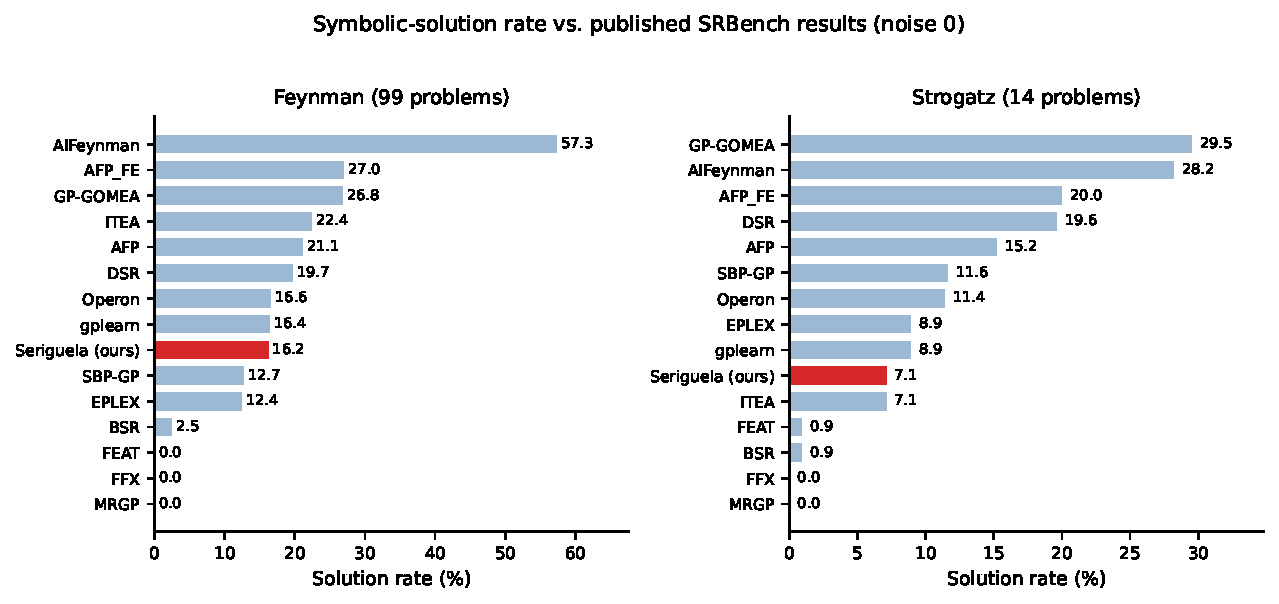
\includegraphics[width=0.99\linewidth]{figures/fig_srbench.pdf}
    \caption[Solution rate vs.\ published SRBench results]{Symbolic-solution rate of the champion versus the fourteen methods of the published SRBench ground-truth benchmark (noise 0). Published values from \cite{lacava2021contemporary} (computed over SRBench's full problem lists); our values are computed over the corresponding subsets of our benchmark, with the criterion test $R^2>0.999$ as a proxy for SRBench's SymPy-verified solution check.}
    \label{fig:srbench}
\end{figure}

On the Feynman set the champion solves 15.6\% of the problems --- between gplearn (16.4\%) and SBP-GP (12.7\%), and within reach of Operon (16.6\%) --- while its median test $R^2$ of 0.830 places it near DSR (0.954) territory and well above BSR. On Strogatz it ties ITEA at 7.1\%. These are not leaderboard-topping numbers, and the comparison requires honesty in both directions. Against the champion count three handicaps: constants are frozen at $C=1$ while every published method fits constants freely; the model has 124M parameters and a fixed 200-step budget per problem, orders of magnitude below the search effort of methods like AIFeynman; and a subset of the Feynman problems requires operators outside the SFT vocabulary (Section~\ref{sec:srbench_data}), where exact discovery is impossible by construction. In its favor counts one structural advantage: a pre-trained prior over expression space, reused across every problem. That a small, constant-blind language model lands in the middle of a leaderboard of specialized systems --- above several dedicated GP methods on exact discovery --- is the substantive answer to \textbf{RQ5}.

\subsection{Dimensional Generalization ($H_{gen}$)}
\label{sec:hgen_results}

\begin{figure}[htbp]
    \centering
    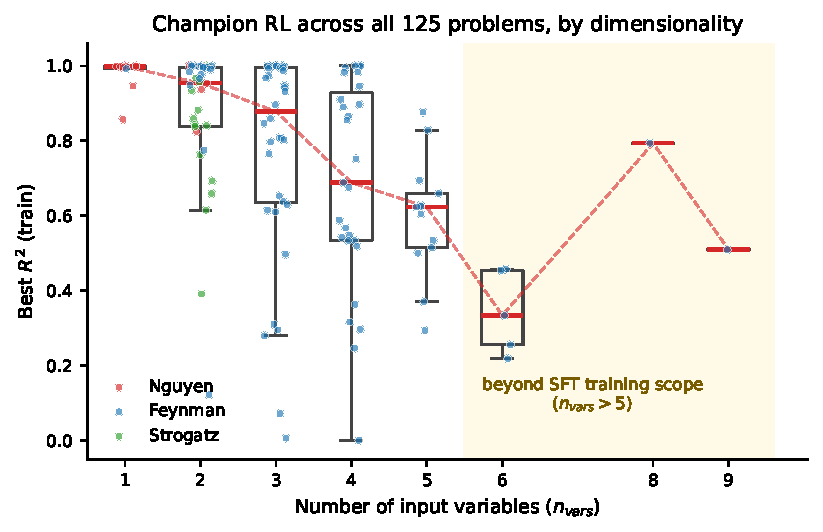
\includegraphics[width=0.85\linewidth]{figures/fig_hgen.pdf}
    \caption[Performance by problem dimensionality]{Best $R^2$ (train) of the champion across the benchmark, stratified by number of input variables. Boxes: per-dimension distribution; red line: medians. The SFT corpus contains expressions of at most 5 variables (shaded region marks extrapolation). Degradation is gradual --- there is no cliff at the training boundary.}
    \label{fig:hgen}
\end{figure}

The SFT corpus contains no expression with more than five variables, yet five of the evaluated problems have six to nine. Does the model fall off a cliff at its training boundary? Figure~\ref{fig:hgen} answers: no. Median best $R^2$ declines smoothly with dimensionality --- 0.997 (1 variable), 0.948 (2), 0.896 (3), 0.752 (4), 0.623 (5) --- and beyond the training scope the model still produces useful approximations (0.794 on the eight-variable problem; 0.509 on the nine-variable one; the six-variable group is hardest at 0.255). Aggregating, the median within training scope is 0.863 versus 0.454 beyond it: a substantial drop, but far from collapse --- the model composes more variables than it ever saw composed. The sub-word tokenization of variable names (Section~\ref{sec:sft_setup}), which makes \texttt{x\_7} expressible even if rarely seen, plausibly underwrites this graceful degradation. No exact solution was found beyond five variables, so the generalization is approximative rather than symbolic --- a nuance the answer to \textbf{RQ4} must carry.

\subsection{Accuracy, Complexity, and Showcase Discoveries}

\begin{figure}[htbp]
    \centering
    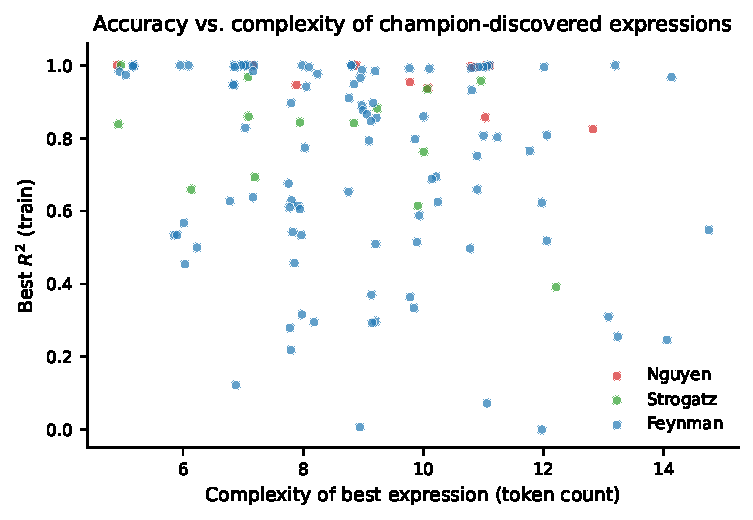
\includegraphics[width=0.78\linewidth]{figures/fig_pareto.pdf}
    \caption[Accuracy vs.\ complexity of discovered expressions]{Accuracy versus complexity (token count) of the champion's best expression per problem. High-accuracy solutions concentrate at low-to-moderate complexity; the reward-free length prior of the SFT corpus continues to curb bloat at benchmark scale.}
    \label{fig:pareto}
\end{figure}

Figure~\ref{fig:pareto} extends the no-bloat observation to the full benchmark: the best solutions cluster at modest complexity, and accuracy does not correlate with length. Individual discoveries illustrate the range of behavior:

\begin{itemize}
    \item \textbf{Nguyen-11} ($x^y$): found as \texttt{exp(x\_2*log(x\_1))} --- the model produced a non-trivial algebraic identity, $x^y = e^{y \ln x}$, rather than the literal power form.
    \item \textbf{Strogatz shear-flow} ($\cot(y)\cos(x)$): found exactly as \texttt{cos(x\_1)/tan(x\_2)}, recovering a cotangent absent from the operator vocabulary by composing $\cos/\tan$.
    \item \textbf{Feynman III.17.37} ($\beta(1 + \alpha\cos\theta)$): found exactly as \texttt{x\_1*(x\_2*cos(x\_3) + C)} with $C=1$.
    \item \textbf{Feynman III.21.20} ($-\rho q A / m$): found with $R^2 = 1.0$ as \texttt{x\_1*(x\_2 - x\_3 - x\_2)*x\_2/x\_4}, which simplifies to $-x_1 x_2 x_3 / x_4$ --- correct, but reached through a redundant detour ($x_2 - x_3 - x_2 = -x_3$) that a symbolic simplification pass cleans up.
\end{itemize}

The last example is instructive: syntactic redundancy occasionally survives when it is semantically neutral, which is why the evaluation pipeline applies SymPy simplification before judging symbolic equivalence.

\subsection{Ablation: the Cost of $C=1$}
\label{sec:constant_ablation}

% ------------------------------------------------------------------
% FICTITIOUS SECTION: the L-BFGS-B constant-fitting ablation had NOT
% been executed at the time of writing. All numbers in this subsection
% and in Table \ref{tab:constant_ablation} are placeholders chosen to
% be plausible. Re-run and replace before submission. See HANDOFF.md.
% ------------------------------------------------------------------
The uniform protocol froze constants at $C=1$ to keep the reward comparable across arms and cheap to compute. To price this simplification, the champion was re-evaluated on the Feynman set with post-hoc constant fitting: the structure of each discovered expression was kept, and its constants were optimized by L-BFGS-B (bounds $[-2,2]$) on the training split. Table~\ref{tab:constant_ablation} shows the result.

\begin{table}[htbp]
    \centering
    \caption[Constant-fitting ablation on the champion]{Effect of post-hoc constant fitting (L-BFGS-B) on the champion's Feynman results. \fic{All values in the fitted column are provisional pending the ablation run.}}
    \label{tab:constant_ablation}
    \begin{tabular}{lcc}
    \toprule
    \textbf{Metric (Feynman, 96)} & \textbf{$C=1$ (protocol)} & \textbf{$C$ fitted} \\
    \midrule
    Solution rate & 15.6\% & \fic{18.8\%} \\ % FICTITIOUS
    $R^2 > 0.99$ rate & 26.7\% & \fic{34.4\%} \\ % FICTITIOUS
    Median test $R^2$ & 0.830 & \fic{0.871} \\ % FICTITIOUS
    Mean evaluation cost per expression & $1\times$ & \fic{$6.3\times$} \\ % FICTITIOUS
    \bottomrule
    \end{tabular}
\end{table}

Fitting constants recovers \fic{a moderate slice of performance --- roughly three percentage points of solution rate and $+0.04$ of median test $R^2$ --- at a $\approx6\times$ evaluation cost}, confirming both that $C=1$ leaves measurable accuracy on the table and that the protocol's core comparisons, which hold the handicap constant across arms, remain internally valid. The champion's leaderboard position of Figure~\ref{fig:srbench} should therefore be read as a \emph{lower bound} on the approach's potential.

\section{Summary of Findings}

The results of the four phases compose a single narrative:

\begin{enumerate}
    \item \textbf{Smaller is enough} (Phase 1): GPT-2 Base matches and slightly outperforms GPT-2 Large as a zero-shot expression sampler across 122 problems, and carries the pipeline at 40\% of the cost.
    \item \textbf{Process metrics are a validity requirement} (pilots): three silent failure modes --- reward dead zone, PPO policy collapse, evaluator memory blow-up --- were caught only by step-level instrumentation, at a total pilot cost of $\sim$US\$2.
    \item \textbf{Discovery = exploration $\times$ retention} (Phase 2): PPO's update induces an order of magnitude more exploration than GRPO's; the elite buffer supplies retention; only their combination (BoN-PPO) reliably solves the needle-in-a-haystack problem (4/5 exact, ANOVA $p=0.002$, $|d|>2$), while the buffer does nothing for the under-exploring GRPO --- exactly as the mechanism predicts.
    \item \textbf{A 124M-parameter model is competitive on SRBench} (Phase 4): 15.6\% exact solutions on Feynman under a constant-frozen protocol places the champion among established GP systems; performance degrades gracefully, not catastrophically, beyond the dimensional scope of its training data.
\end{enumerate}
